\documentclass{cmpstyle}
\title{UG06 Group Report}
\author{UG06}
\usepackage{graphics}
\usepackage{hyperref}
\begin{document}
\section{Group members}
Andrew Sturdy - 100318044\newline
Thomas\newline
Tan
\section{Privacy and ethics}

\section{Mitigations}

\subsection{SQL Injection}
%What was coded
%Usability
%Any prebuilt libraries
SQL Injection is when SQL code is ran on a website via a textbox or entry field. The way we have mitigated this is by using parametrised queries wherever the user inputs data for a query. A parametrised query is a query that "drops in" the variables instead of using string concatenation. Because the values are not added on the end and are instead dropped in, the user has no way of terminating the query to run their own code. We used the node library "pg" to communicate with the database, this library had built in support for parametrised queries so no other library was needed. These queries function the same as normal queries and run at similar speeds to normal ones meaning the user wont notice the difference. As this is all happening server side it will have no direct impact on usability, however if these queries were to run slow then the user would notice.
\subsection{Account Enumeration}
%What was coded
%Usability
%Any prebuilt libraries
Account Enumeration is when a user iterates through a dictionary of possible username and uses the response from the server to determine if that username is in use or not. The way we have prevented this is by making the response from the server the same whether the username or the password is incorrect making it hard to tell which one if any were correct. We have also made the timing of the responses the same so that they can not be told apart that way, this was done by running through the entire login process no matter whether the username or password was correct. This can have an impact on usability as it can make the process of forgetting login information slower and less informative, if you forget your credentials the website wont tell you which of them you got right which can be frustrating for users.
\subsection{Cross-site Scripting}
Cross-site Scripting is when code is injected into a website to then be executed later, this typically happens in the form of html and JavaScript code that gets issued to a text form to run when its displayed later. The way we have mitigated this is through html encoding, all of the html characters ($<$,$>$,",\,\&) needed to write code have special characters that represent them so websites can display them safely, we use this when displaying posts as its the only time code could be injected to run later. Before the posts are displayed on the screen they all go through a function that converts html characters to their display counterparts so $<$ becomes \&lt while being ran but will display as $<$. This should have little to no affect on usability as the users wont see the converted characters and the process is very fast so it should not be much slower than if we didn't do it.
\subsection{Cross-site Request Forgery}
\subsection{Session Hijacking}
\subsection{Hashing, Salting and Encryption}
The passwords of each user is salted with their user id allowing their passwords to be distinct when hashed even if they were originally the same password. The reason the user id was chosen is because the hashes needed to repeatable as the user id is something unique to the user that is accessible to the server.

Hashing was used on user's passwords before they were entered into the database, we used SHA-128 as our hashing algorithm, which is the 128 bit version of SHA-1. This hashing algorithm was implemented using a pre-built library called jssha which adds functions to hash using most versions of SHA. We chose SHA-128 because it produces strong but small hashes. As this web blog should not contain a lot of personal information there is no need for very strong security.

The encryption we used was AES-128-cbc which uses a 128 bit key size and performs 10 rounds of encryption. We use this algorithm in cipher block chain mode (cbc) which allows the output of the encryption to be of fixed sizes as cbc causes the data to be padded to the block size. All user data that enters the database is encrypted but the post data is not. Posts are not encrypted as they should contain no data about the user and encrypting data that does not need to be would slow down the flow of the website as all posts would need to be decrypted to be displayed.

 
\section{Authentication methods}	
	
\section{Testing}
\subsection{Think Aloud Testing}
Think aloud testing is when users are handed the product, in this case the website, and asked to perform a series of tasks, they are monitored during this and their progress is recorded along with any issues they encounter. This type of testing is for usability and is typically performed in 3 or more rounds, you would record the results of people in different demographics and using the notes make improvements, after the improvements a new group of people from the same demographics would use the site.

The tasks the users where asked to perform where:
\begin{itemize}
	\item Register an account
	\item Make a post
	\item Log out
	\item Log in
	\item View the post you made
	\item View all available posts
\end{itemize}
These tasks where performed in the order listed and allowed us to test all aspects of our site individually. We tested on 3 different demographics, young male university students, young female sixform students and female adults. 

The young male managed to create an account with ease and make a post, however he noted that the website gives a lack of information on whether the post was successfully made or not causing this task to take longer than expected. He had no problems logging out and then back in, he tried to search for the category his post was under however our search bar only works based off of title so it didn't work. To view all posts he simple pressed buttons on the screen around the search bar and happened to press the search button while the bar was empty which shows every post. Overall he did not find it easy to use due the lack of feedback the site gives on whether actions are successful or not. The table of results for this test can be found in Figure \ref{YMale}.

The young female did not like the 2 factor authentication used as it required a new app on their phone. She had no issues until tasked with viewing all posts, after a couple of minutes of looking they gave up. The table of results for this can be found in Figure\ref{YFemale}.

The adult female had the same issues as the young male, they didn't know if the test was successfully made and they did not easily find the way to search for all posts. The table of results can be found in Figure\ref{Female}.
\subsection{Unit Testing}
This website was thoroughly tested using unit tests, these tests where carried out throughout development and also at the end. The final test results can be found in figure\ref{Testing} and it shows that all but 2 test were passed. The two tests that did not pass are failing two factor authentication (test 30) and Searching for something that does not exist (test 32). In both cases the behaviour demonstrated is valid however the user is not informed. If you get the two factor authentication code wrong at log in or registration it does not tell the user this but it does not log the user in either. If the user searches for a title that has no results, the user is not told that nothing could be found but nothing is displayed either.
\clearpage
\appendix
\begin{figure}[htb]
	\centering
	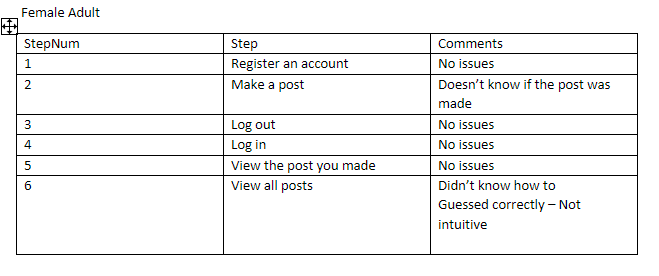
\includegraphics[width=0.75\textwidth]{Female.png}
	\caption{Female Adult \label{Female}}
\end{figure}
\begin{figure}[htb]
	\centering
	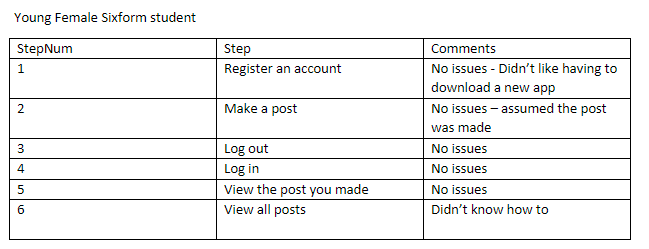
\includegraphics[width=0.75\textwidth]{Young female.png}
	\caption{Young Female Student \label{YFemale}}
\end{figure}
\begin{figure}[htb]
	\centering
	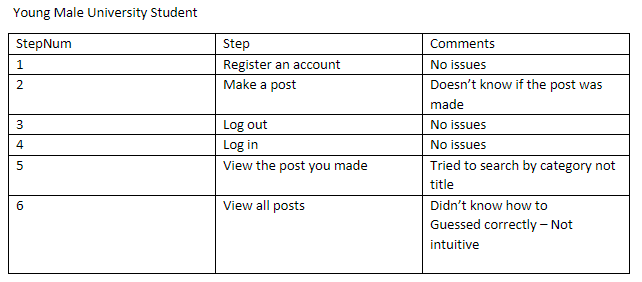
\includegraphics[width=0.75\textwidth]{Young male.png}
	\caption{Young Male Student \label{YMale}}
\end{figure}
\begin{figure}[htb]
	\centering
	\caption{Unit Testing plan/results \label{Testing}}
	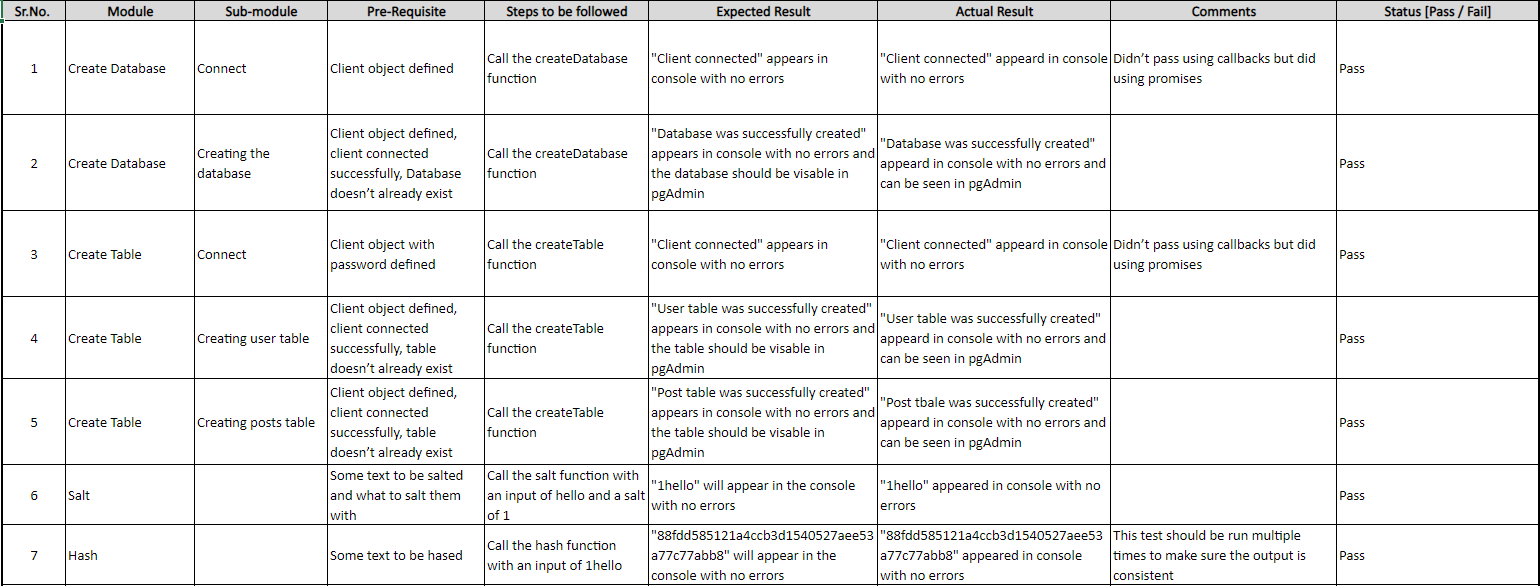
\includegraphics[width=0.75\textwidth]{Testing1.png}
\end{figure}
\begin{figure}[htb]
	\centering
	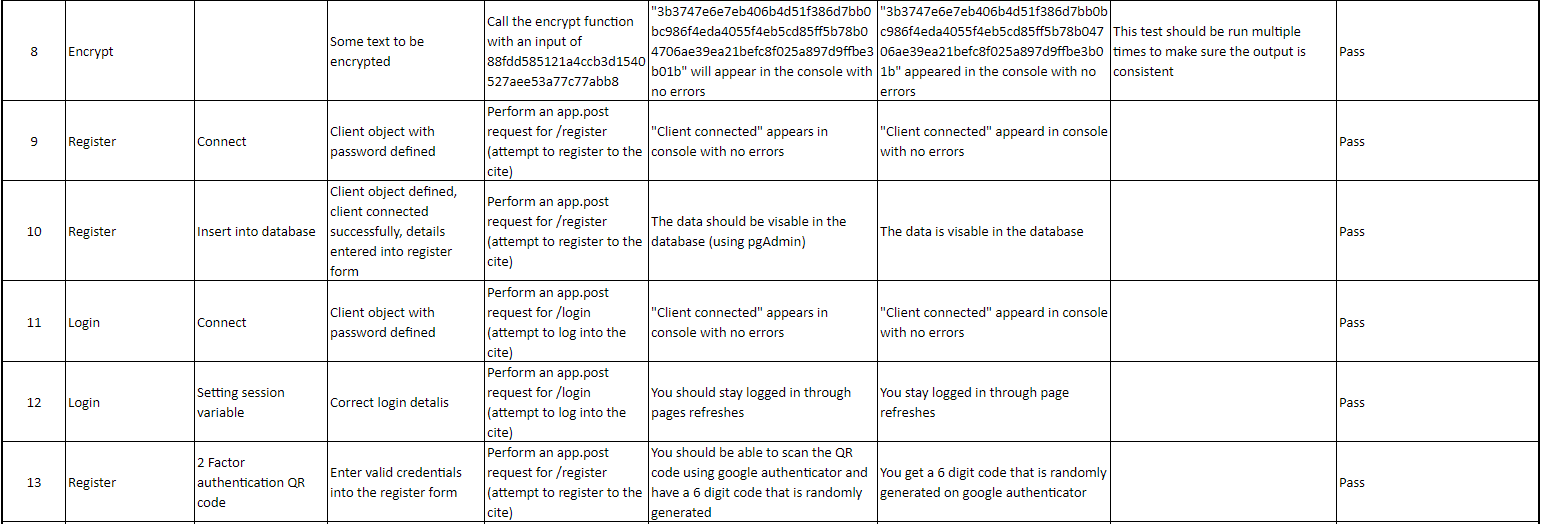
\includegraphics[width=0.75\textwidth]{Testing2.png}
\end{figure}
\begin{figure}[htb]
	\centering
	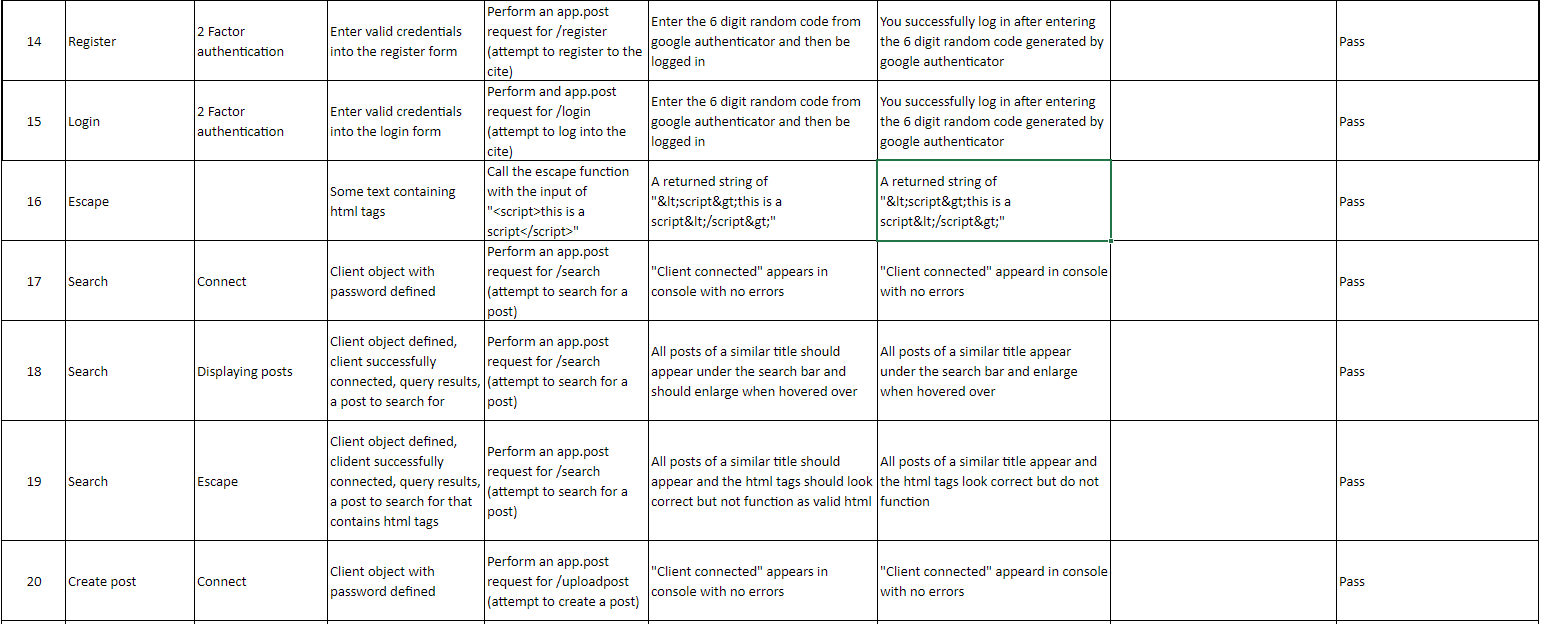
\includegraphics[width=0.75\textwidth]{Testing3.png}
\end{figure}
\begin{figure}[htb]
	\centering
	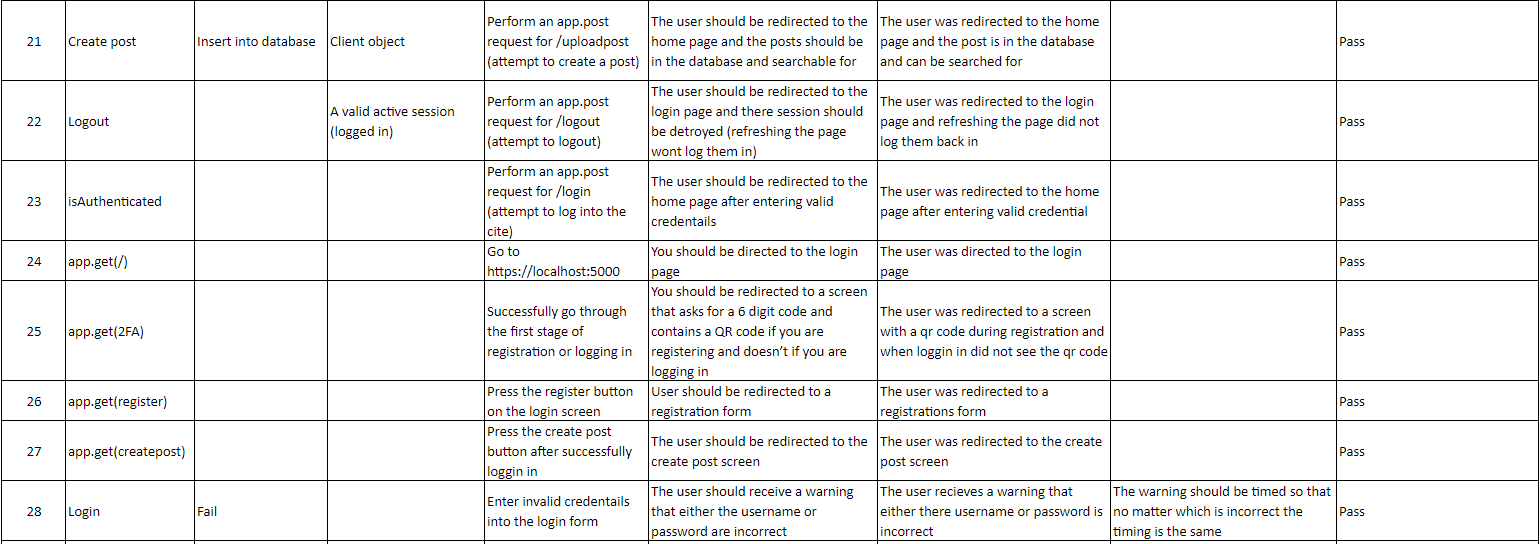
\includegraphics[width=0.75\textwidth]{Testing4.png}
\end{figure}
\begin{figure}[htb]
	\centering
	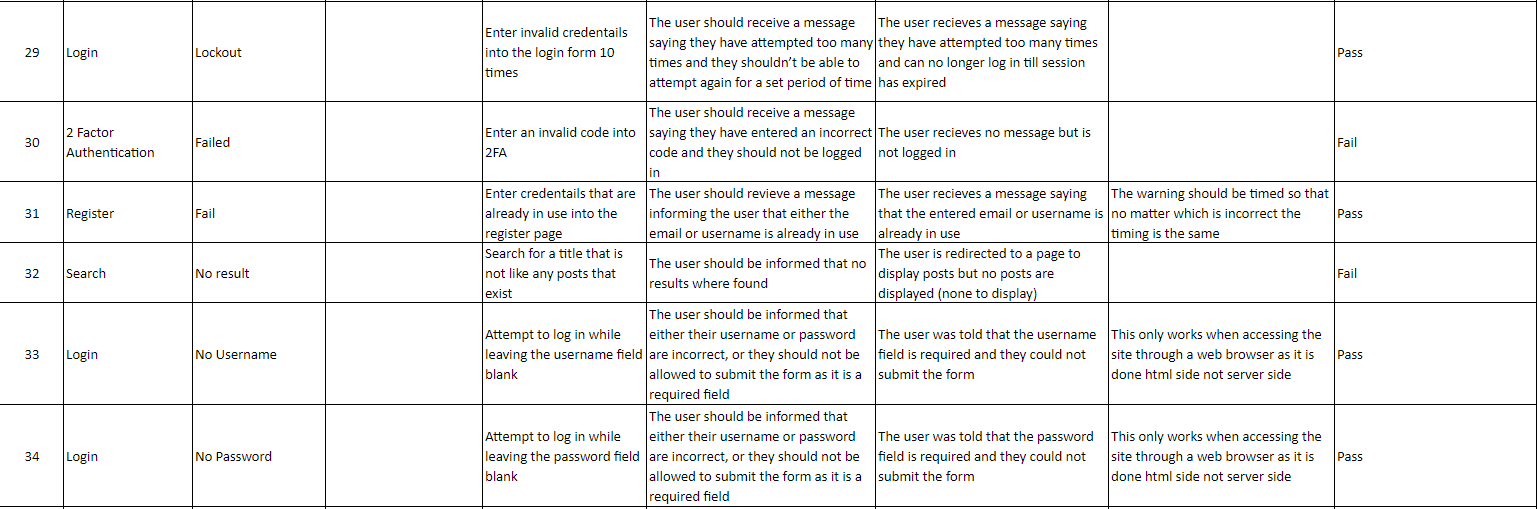
\includegraphics[width=0.75\textwidth]{Testing5.png}
\end{figure}
\begin{figure}[htb]
	\centering
	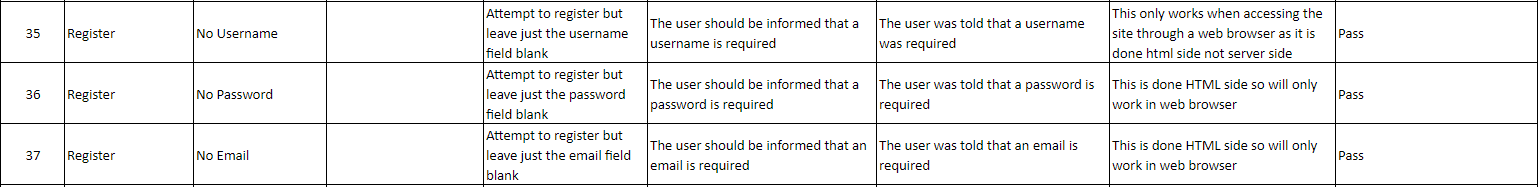
\includegraphics[width=0.75\textwidth]{Testing6.png}
\end{figure}
\end{document}